
\section{Introduction}
\begin{figure}[t]
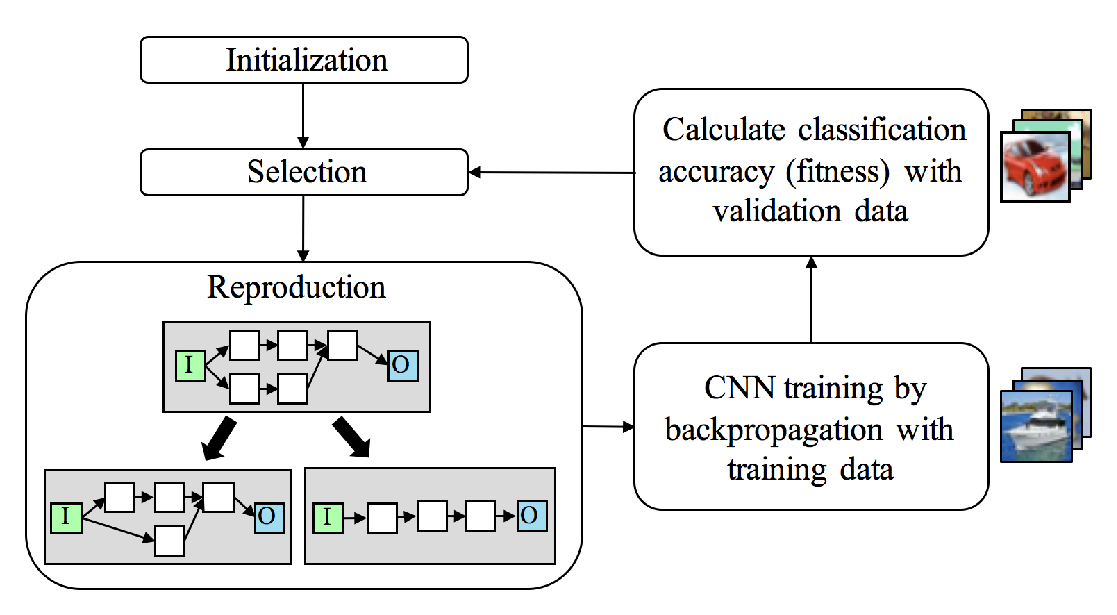
\includegraphics[scale=0.65]{images/overview.eps}
\caption{Overview of our method. Our method searches a CNN architecture using genetic programming. That CNN architecture is then trained on a learning task, and returns an accuracy. The network search is performed to maximize the accuracy by the evolutionary algorithm. \shin{I cannot understand above figure...}}
\label{overview}
\end{figure}

\begin{figure*}[t]
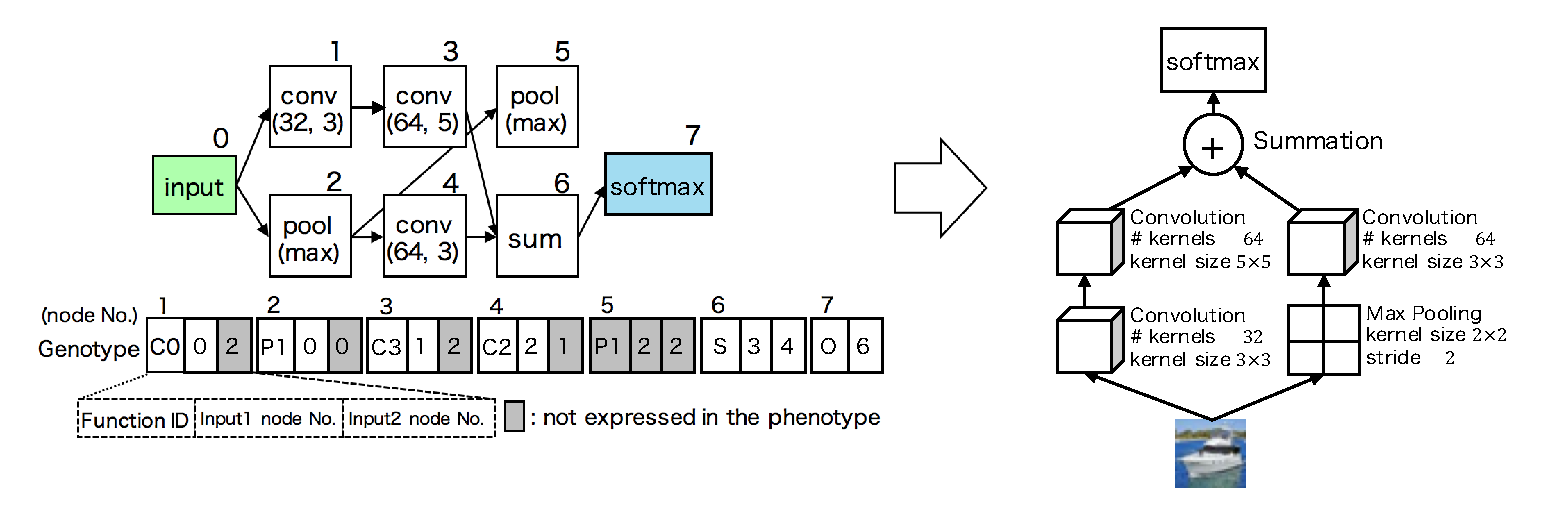
\includegraphics[scale=0.7]{images/genotype.eps}
\caption{Example of a genotype and a phenotype. The genotype (Left) defines a CNN architecture (Right).}
\label{genotype}
\end{figure*}

\new{Deep learning, which uses deep neural networks as a model, has shown a surprising performance on many challenging artificial intelligence and machine learning tasks such as image recognition \cite{lecun_gradient-based_1998,krizhevsky_imagenet_2012}, speech recognition \cite{hinton_deep_2012}, and reinforcement learning tasks \todo{ref. of DQN}.}
In particular, convolutional neural networks (CNNs) \cite{lecun_gradient-based_1998} have seen huge success in image recognition tasks in the last few years \new{and is applied to various computer vision tasks \todo{ref. e.g. GAN, colorization, image to text anotation...}.}
A \new{commonly used} CNN architecture mainly consists of several convolutions, pooling, and fully connected layers.
\new{Several recent studies focus on developing the novel CNN architecture that achieves higher classification accuracy, e. g., GoogleNet \cite{szegedy_going_2015}, ResNet \cite{he_deep_2016}, and DensNet \todo{ref.}.}
Despite their success, designing CNN architectures is still a difficult task \new{since there exist many design parameters such as the depth of a network, the type and parameters of each layer, and the connectivity of the layers.}
\new{The state-of-the-art CNN architectures have become deep and complex, which suggests that a significant number of design parameters should be tuned to realize the best performance for a specific dataset.
Therefore, the trial and error or expert knowledge are required when the users construct the suitable architecture for their target dataset.
Because of this situation, the automatic design methods for the CNN architectures is highly beneficial.}

\new{The neural network architecture design can be viewed as the model selection problem in the machine learning. The straight-forward approach is to deal with the architecture design as the hyperparameter optimization problem, optimizing the hyperparameters such as the number of layers and neurons using black-box optimization techniques \cite{}.}

\new{Evolutionary computation has been traditionally applied to design the neural network architectures \todo{ref. X. Yao's review, Kitano, etc...}.
There are two types of encoding schemes for the network representation: direct and indirect coding.
The direct coding represents the number and connectivity of neurons directly as the genotype, whereas the indirect coding represents a generation rule of the network architectures.
While almost traditional approaches optimize the number and connectivity of low-level neurons, the modern neural network architectures for deep learning have many units and various types of units, e.g., convolution, pooling, and normalization.
Optimizing those many parameters in reasonable computational time may be difficult.
Therefore, the use of the highly-functional modules as a minimum unit is promising.}

\shin{This paragraph will move to sect. 2.}
Genetic algorithms (GA) based approaches have been used to optimize architectures of neural networks \cite{schaffer_combinations_1992}.
Fernando et al. \cite{fernando_convolution_2016} have proposed the differentiable pattern producing networks (DPPN) to optimize weights of a denoising autoencoder.  
The DPPN is a differentiable version of the compositional pattern producing networks (CPPN) \cite{stanley_compositional_2007}.
While the DPPN showed a good performance on image reconstruction tasks, this method is still limited in fixed-length models defined by hand.
Verbancsics et al. \cite{verbancsics_generative_2013} \cite{verbancsics_image_2015} have designed artificial neural networks and CNN architectures with the hypercube-based neuroevolution of augmenting topologies (HyperNEAT) \cite{stanley_hypercube-based_2009}.
However, to the best of our knowledge, these networks designed with HyperNEAT have failed to match the performance of state-of-the-art methods.
Also, these methods deal with the architectures defined by human experts, thus it is hard to design neural network architectures from scratch.

\new{In this paper, we attempt to design CNN architectures based on a genetic programming.
We use the Cartesian genetic programming (CGP) \cite{miller_cartesian_2000,harding_evolution_2008} encoding scheme, one of the direct encoding, to represent the CNN structure and connectivity.
The advantage of this representation is its flexibility; it can represent variable-length network structure and the skip connections.
Moreover, we adopt the relatively highly-functional modules such as convolutional blocks and tensor concatenation as the node functions in CGP to reduce the search space.
To evaluate the architecture represented by the CGP, we train the network using training dataset in an ordinary way. Then the performance for another validation dataset is assigned as the evaluation of the architecture. Based on this fitness evaluation, an evolutionary algorithm optimizes the CNN architectures.
 To check the performance of the proposed approach, we conducted the experiment constructing the CNN architecture for the image classification task with the CIFAR-10 dataset \cite{krizhevsky_learning_2009}. The experimental result shows that the proposed approach can automatically find the competitive CNN architecture compared with state-of-the-art models.}

\new{The rest of this paper is organized as follows. The next section presents related work on the neural network architecture design. In Section 3, we describe our genetic programming approach to design the CNN architectures. We test the performance of the proposed approach through the experiment. Finally, in Section 5, we describe our conclusion and future work.}

\shin{Checked up to here.}

\section{Related work}
Automating neural network design and hyperparameter optimization are important topic in machine learning.
This section briefly reviews these research areas.

\subsection{Hyperparameter optimization}
For hyperparameter optimization, there are many methods such as grid search, gradient search \cite{bengio_gradient-based_2000}, random search \cite{bergstra_random_2012}, and Bayesian optimization based methods \cite{hutter_sequential_2011}, \cite{snoek_practical_2012}.
Recently, Bayesian optimization methods have shown a good performance in several datasets.
Bergstra et al. \cite{bergstra_algorithms_2011} have proposed the Tree-structured parzen estimator (TPE) and shown better results than manual search and random search \cite{bergstra_random_2012} in the hyperparameter optimization task.
Also, Bergstra et al. \cite{bergstra_making_2013} have proposed a meta-modeling approach based on the TPE for supporting automated hyperparamter optimization. 
While models based on the gaussian process are generally used for Bayesian optimization, gaussian process based approaches have a problem of increasing inference time cubically in the number of observations.
To solve this problem, Snoek et al. \cite{snoek_scalable_2015} have replaced the gaussian process with a deep neural network, which improved its scalability.

While these methods have seen success, these methods are limited in fixed-length architectures, i.e., it is difficult to design variable-length architectures from scratch.

\subsection{Designing neural network architectures}
Recently studies on automating neural network design using reinforcement learning have been made \cite{zoph_neural_2016} \cite{baker_designing_2016}.
These studies showed that a reinforcement learning based method is able to generate good CNN architectures for image classification tasks.
In \cite{zoph_neural_2016}, a recurrent neural network (RNN) is used to generate the neural network architecture, and the RNN is trained with reinforcement learning to maximize the expected accuracy on a learning task.
To accelerate training, this method uses distributed training and asynchronous parameter updates with $800$ GPUs.
Baker et al. \cite{baker_designing_2016} have proposed a meta-modeling approach based on reinforcement learning to compose CNN architectures.
A Q-learning agent explores and exploits a space of model architectures with an $\epsilon -$greedy strategy and experience replay.

Unlike these approaches, our method adopts a genetic programming based approach to design CNN architectures.
In addition, we introduce a highly-functional modules such as convolutional blocks and tensor concatenations in order to effectively find better CNN architectures.

\section{Designing CNN architectures using genetic programming}
Our method represents a CNN architecture as a feedforward network structure that is defined by the CGP.
The CNN architecture defined by the CGP is trained on a learning task, and the network is optimized to maximize the validation accuracy by the evolutionary algorithm.
In the following section, we will describe how CNN architectures can be designed and optimized with the CGP in detail.

\subsection{Designing CNN architectures with the CGP}
We use a feedforward network that consists of $R$ rows by $C$ columns, i.e., the number of intermediate nodes of the network is $R\times C$.
Figure \ref{genotype} shows an example of the network of two rows by three columns and its genotype and phenotype.
A type of each node is represented as four different types of layers: convolution, pooling, summation, and concatenation.
The detailed parameters for each layer are shown in Table \ref{layer_param}.
The convolution node consists of a standard convolution processing with batch normalization \cite{ioffe_batch_2015} and rectified linear units \cite{nair_rectified_2010}.
The pooling node consists of the standard max pooling and average pooling processing.
The summation node performs element-wise addition of two feature maps, channel by channel. 
If input feature maps to be added have different sizes, we pad the small feature map with zeros for increasing dimensions.
The concatenation node concatenates two feature maps in the depth dimensions.
If input feature maps to be concatenated are different sizes, we pad the small feature map with zeros.
Adding these summation and concatenation nodes to the network architecture allow our method to generate shortcut connections or branching layers such as GoogleNet \cite{szegedy_going_2015} and Residual Net \cite{he_deep_2016}.

The CGP inter-connectivity is determined by the levels back parameter $l$, which decides nodes of how many previous columns to connect to nodes in the current column, i.e., each node can have one or two connections to nodes in the $l$ previous columns.
Note that nodes in the same column are prohibited to be connected to each other.
The types and connections of nodes are optimized by the evolutionary algorithm.

\begin{table}[tb]
  \caption{Parameter details for each layer}
  \label{layer_param}
  \begin{tabular}{l|l|l} \hline
    Node type & Parameters & Values or description \\ \hline
    Convolution & Kernel size & $\in \{3\times 3, 5\times 5\}$ \\ 
                        & \# kernels & $\in \{32, 64, 128\}$ \\ 
                       & Stride & $1$ \\ 
                       & \# inputs & $1$ \\ \hline
      Pooling     & Kernel size & $2\times 2$ \\ 
                       & Stride & $2$ \\ 
                       & \# inputs & $1$ \\ \hline
     Summation & \# inputs & $2$ \\ 
                         &                & Element-wise addition. \\ \hline
 Concatenation & \# inputs & $2$ \\ 
                      &  & Concatenate in the \\
                       &  & depth dimension.\\  \hline
  \end{tabular}
\end{table}

\subsection{Optimization of the CGP}
We use mutation as a genetic operator.
The mutation operator is applied to one individual as follows:
\begin{itemize}
  \item Select several nodes with probability $\epsilon$ for each node.
  \item Change the type and connectivity of the selected nodes randomly.
\end{itemize}
Note that we apply the mutation operator to nodes until one or more active nodes that are associated with the output path are changed.
As training a CNN can take hours, we apply the above mutation operator to save time.

We use a simple form of $(1+\lambda)$ evolutionary strategy (with $\lambda = 2$) to design CNN architectures.
The algorithm is as follows:
\begin{description}
  \item[1.] Generate an initial individual at random as a parent $M$, and train the CNN defined by $M$.
  \item[2.] Generate a set of two offsprings $C$ by applying the mutation operation to $M$.
  \item[3.] Train these two CNNs defined by offsprings $C$.
  \item[4.] Select an elite individual from the set of $M$ and $C$, and replace $M$ with the elite individual.
  \item[5.] Return to step $2$ until a stopping criterion is satisfied.
\end{description}
We employ the accuracy of the CNN on a validation set as the fitness of each individual.

\section{Experiments and Results}
\subsection{Dataset}
We test our method to the image classification task with CIFAR-10 dataset which has $10$ classes with $50,000$ training images and $10,000$ test images.
We sampled $5,000$ images randomly from the training set for the validation set, the remaining $45,000$ images are the training set.
In this experiment, we use data preprocessing and augmentation procedure.
We first preprocess the data with the per-pixel mean subtraction.
We then pad $4$ pixels on each side, and choose a random $32\times 32$ crop from the padded image.
At last, we perform random horizontal flips on the cropped $32 \times 32$ image. 
\subsection{Training details}

\begin{table}[tb]
  \caption{Parameter settings for the CGP}
  \label{cgp_param}
  \begin{tabular}{l|l} \hline
    Parameters & Values or description \\ \hline
   \# Generations & $300$ \\ 
   Mutation rate & $0.05$ \\
   \#  Rows & $5$ \\
   \#  Columns & $30$ \\
   Levels back & $10$ \\
   Generation alternation model & $(1+2)$ Evolution Strategy \\ \hline
  \end{tabular}
\end{table}

Parameter settings for the CGP is shown in Table \ref{cgp_param}.
Once the CGP samples a CNN architecture, every CNN is trained for $50$ epochs with the Adam optimizer \cite{kingma_adam:_2015} with an initial learning rate of $0.01$.
We reduce the learning rate by a factor of $10$ every $20$ epochs.
All weights of CNN are initialized with He \cite{he_delving_2015}, and the batch size is $128$.

After finishing the evolution of the CGP, we select the architecture that showed the best validation accuracy.
We then fine-tune the best model with a different training schedule.
During this phase, we set a learning rate to $0.01$ for $50$ epochs, then $0.001$ for $50$ epochs.
The other parameters are unchanged.
After training the best model, we apply the model to the test set.

\subsection{Results}


\section{Conclusions}